\documentclass[mathserif, handout]{beamer}

\usepackage{url}
% ======================================================================
% General LaTeX Setup for Beamer (Reusable Preamble)
% Author: Chandra Gummaluru
% ======================================================================

\documentclass[mathserif, handout]{beamer}
\setbeamertemplate{frametitle}{}

% ------------------------------------------------------------
% basic packages
% ------------------------------------------------------------
\usepackage{url}
\usepackage{ifthen}
\usepackage{enumerate}
\usepackage[font=small]{caption}
\usepackage{subcaption}
\usepackage{moresize}
\usepackage[outline]{contour}
\usepackage{transparent}
\usepackage{worldflags}
\usepackage{bm}
\usepackage{graphbox}
\usepackage{mathtools}
\usepackage{multirow}
\usepackage{fontawesome5}
\usepackage{pifont}
\usepackage{array}
\usepackage{comment}

% ------------------------------------------------------------
% math
% ------------------------------------------------------------
\DeclarePairedDelimiter{\floor}{\lfloor}{\rfloor}
\DeclarePairedDelimiter{\ceil}{\lceil}{\rceil}

% ------------------------------------------------------------
% colors
% ------------------------------------------------------------
\definecolor{hl}{RGB}{248,196,69}
\definecolor{myred}{HTML}{ED5565}
\definecolor{myorange}{HTML}{FC6E51}
\definecolor{myyellow}{HTML}{FFCE54}
\definecolor{mycyan}{HTML}{4FC1E9}
\definecolor{myblue}{HTML}{5D9CEC}

\newcommand{\graytext}[1]{\footnotesize\color{gray}#1\normalsize\color{black}}

% ------------------------------------------------------------
% symbols
% ------------------------------------------------------------
\newcommand{\cmark}{\ding{51}}
\newcommand{\xmark}{\ding{55}}

% ------------------------------------------------------------
% highlighting
% ------------------------------------------------------------
\newcommand{\reducedstrut}{\vrule width 0pt height .9\ht\strutbox depth .9\dp\strutbox\relax}
\newcommand{\highlight}[1]{%
  \begingroup\setlength{\fboxsep}{0pt}\colorbox{hl}{\reducedstrut$\displaystyle #1$\/}\endgroup}
\newcommand{\highlightc}[2]{%
  \begingroup\setlength{\fboxsep}{0pt}\colorbox{#1}{\reducedstrut$\displaystyle #2$\/}\endgroup}

% ------------------------------------------------------------
% environments (boxes)
% ------------------------------------------------------------
\usepackage{tcolorbox}
\tcbuselibrary{skins}

\newtcolorbox{thmbox}[1][]{colback=gray!30!white!20, colframe=black, fonttitle=\bfseries, title=#1, boxrule=0.5pt}

% 1) Bottom open (draw top + sides only)
\newtcolorbox{thmboxtop}[1][]{
    enhanced,
    frame hidden,
    colback=gray!30!white!20,
    borderline north={0.5pt}{0pt}{black}, % top
    borderline west={0.5pt}{0pt}{black},  % left
    borderline east={0.5pt}{0pt}{black}   % right
}

% 2) Top open (draw bottom + sides only)
\newtcolorbox{thmboxbot}[1][]{
    enhanced,
    frame hidden,
    colback=gray!30!white!20,
    borderline south={0.5pt}{0pt}{black}, % bottom
    borderline west={0.5pt}{0pt}{black},  % left
    borderline east={0.5pt}{0pt}{black}   % right
}

% 3) Side only (draw only left and right)
\newtcolorbox{thmboxside}[1][]{
    enhanced,
    frame hidden,
    colback=gray!30!white!20,
    borderline west={0.5pt}{0pt}{black},  % left
    borderline east={0.5pt}{0pt}{black}   % right
}

\newtcolorbox{defboxtop}[1][]{
    enhanced,
    colback=gray!30!white!20,
    frame hidden,
    overlay={
        % Draw top + sides with rounded corners
        \draw[line width=0.5pt, black, rounded corners=3mm]
            (frame.south west) -- (frame.north west) -- (frame.north east) -- (frame.south east);
    },
    #1
}

\newtcolorbox{defboxbot}[1][]{
    enhanced,
    colback=gray!30!white!20,
    frame hidden,
    overlay={
        % Draw top + sides with rounded corners
        \draw[line width=0.5pt, black, rounded corners=3mm]
            (frame.north west) -- (frame.south west) -- (frame.south east) -- (frame.north east);
    },
    #1
}

\newtcolorbox{defboxside}[1][]{
    enhanced,
    frame hidden,
    colback=gray!30!white!20,
    borderline west={0.5pt}{0pt}{black},  % left
    borderline east={0.5pt}{0pt}{black}   % right
}

\newtcolorbox{proofbox}[1][]{colback=gray!20!white!20, colframe=grey, fonttitle=\bfseries, title=#1, boxrule=0.5pt, colbacktitle=white, enhanced jigsaw, sharp corners}

% ------------------------------------------------------------
% code listings
% ------------------------------------------------------------
\usepackage{listings}
\lstdefinestyle{mypython}{
  language=Python,
  deletekeywords=[2]{open, next, from, chr, str, int},
  morekeywords=[3]{List, Graph, Tree, Dict, Set, UnionFind, Ordict, Trie, Queue},
  morekeywords=[4]{ListNode, Vertex, Edge, Path, TreeNode, DictNode, UnifNode, OrdictNode, TrieNode, QueueNode},
  morekeywords=[5]{True, False, Boolean, String, Integer, Key, Function, KeyedObject, Object, Array, Tuple, Optional, None},
  keywordstyle=\color{mycyan}\bfseries,
  keywordstyle=[3]\color{myblue}\bfseries,
keywordstyle=[4]\color{myblue}\bfseries,
keywordstyle=[5]\color{mycyan}\bfseries,
  stringstyle=\color{orange},
  commentstyle=\color{gray}\itshape,
  basicstyle=\ttfamily\footnotesize,
  numbers=left,
  numberstyle=\tiny\color{gray},
  stepnumber=1,
  numbersep=5pt,
  xleftmargin=15pt,
  frame=none,
  showstringspaces=false,
  breaklines=true,
  breakatwhitespace=true,
  tabsize=4,
  columns=flexible
}


% ------------------------------------------------------------
% algorithms
% ------------------------------------------------------------
\usepackage{algorithm}
\usepackage[endLComment=~]{algpseudocodex}
\makeatletter
\algrenewcommand\ALG@beginalgorithmic{\footnotesize}
\makeatother

% ------------------------------------------------------------
% optimization environments
% ------------------------------------------------------------
\usepackage[nocomma]{optidef}

% ------------------------------------------------------------
% pgfplots and pie charts
% ------------------------------------------------------------
\usepackage{pgfplots}
\usepackage{pgf-pie}
\pgfplotsset{compat=1.7}

% ------------------------------------------------------------
% tikz
% ------------------------------------------------------------
\usepackage{tikz}
\usetikzlibrary{
  angles, quotes, positioning, fit, backgrounds, shapes.geometric, intersections,
  calc, shapes, mindmap, decorations.text, arrows, arrows.meta,
  automata, chains, decorations.pathreplacing, calligraphy,
  decorations.markings, shapes.misc, decorations.pathmorphing
}
\tikzset{
  invisible/.style={opacity=0},
  visible on/.style={alt=#1{}{invisible}},
  alt/.code args={<#1>#2#3}{\alt<#1>{\pgfprioritysalso{#2}}{\pgfprioritysalso{#3}}}
}

\newcommand{\multiedge}[5][]{
\pgfmathsetmacro{\N}{#4}
\pgfmathsetmacro{\mid}{(\N-1)/2}
\foreach \i in {0,...,\numexpr#4-1\relax} {

\pgfmathsetmacro{\k}{\i-\mid}
\draw[#1] ($ (#2) + \k*#5*($(#2)!1!90:(#3)$) $) -- ($ (#3) + \k*#5*($(#2)!1!90:(#3)$) $); 

}
\draw[#1,  -{>[scale=1]}]
  ($(#2)!0.54!(#3)$) -- ($(#2)!0.55!(#3)$);
}

% ------------------------------------------------------------
% bibliography
% ------------------------------------------------------------
\usepackage[style=ieee]{biblatex}
\setbeamertemplate{bibliography item}{\insertbiblabel}
\setbeamertemplate{background canvas}{
  \begin{tikzpicture}[remember picture,overlay]
    \node[opacity=0.0075]
      at (current page.center)
      {
\includegraphics[width=0.8\paperwidth]{images/signature.pdf}};
  \end{tikzpicture}
}

% ------------------------------------------------------------
% beamer theme and settings
% ------------------------------------------------------------
\usetheme{Boadilla}
\usecolortheme{seagull}
\beamertemplatenavigationsymbolsempty
\setbeamertemplate{enumerate item}{(\arabic{enumi})}
\setbeamertemplate{enumerate subitem}{(\alph{enumii})}
\setbeamertemplate{enumerate subsubitem}{(\roman{enumiii})}
\setbeamertemplate{itemize item}[circle]
\setbeamertemplate{itemize subitem}{\circ}
\setbeamertemplate{itemize subsubitem}{-}
\setbeamercolor{item}{fg=black!40}
\setbeamercovered{transparent=10}

% ===========================
% Premade TikZ Figure Commands
% ===========================

% images w/ labels
% inside tikz as a node
\NewDocumentCommand{\labeledimgnodetikz}{O{} m m m m m m}{%
	\begin{scope}[transparency group, #1]
		\node[
			draw,
			circle,
			inner sep=0,
			outer sep=0,
			minimum size=10mm,
			#1
		] (#5) at (#3,#4)
		{\includegraphics[scale=#7]{#6}};
		\node[
			rectangle,
			draw=black,
			thick,
			fill=black!55,
			rounded corners=0.1mm,
			inner sep=0pt,
			outer sep=0pt,
			minimum size=2.8mm,
			minimum width=3.5mm
		] at (#3,#4-0.1) {};
		\node[outer sep=0, inner sep=0, white] at (#3,#4-0.1) {\footnotesize #2};
	\end{scope}
}

% inside tikz isolated

% outside tikz
\NewDocumentCommand{\labelednode}{m}{%
	\begin{tikzpicture}[baseline={(0,-1mm)}]
		\node[
			rectangle,
			thick,
			draw=black,
			fill=black!55,
			rounded corners=0.1mm,
			inner sep=0pt,
			outer sep=0pt,
			minimum size=2.8mm,
			minimum width=3.5mm
		] at (0,0) {};
		\node[outer sep=0, inner sep=0, white, minimum size=2.8mm, minimum width=3.5mm] at (0,0) {\footnotesize #1};
	\end{tikzpicture}
}

% images only
% inside tikz as a node
\NewDocumentCommand{\imgnodetikz}{O{} m m m m m m}{%
	\begin{scope}[transparency group, #1]
		\node[
			draw,
			circle,
			inner sep=0,
			outer sep=0,
			minimum size=10mm,
			#1
		] (#5) at (#3,#4)
		{\includegraphics[scale=#7]{#6}};
		\node[
			rectangle,
			draw,
			thick,
			fill=black!55,
			rounded corners=0.1mm,
			inner sep=0pt,
			outer sep=0pt,
			minimum size=2.8mm,
			minimum width=3.5mm,
			opacity=0
		] at (0,0) {};
		\node[outer sep=0, inner sep=0, white, opacity=0] at (0,0) {\footnotesize #2};
	\end{scope}
}

% inside tikz isolated
\NewDocumentCommand{\imgtikz}{O{} mm}{%
	\begin{scope}[transparency group, #1]
		\node[
			inner sep=0,
			outer sep=0
		] (#5) at (#3,#4)
		{\includegraphics[scale=#3]{#2}};
	\end{scope}
}


% outside tikz
\NewDocumentCommand{\imgnode}{mm}{%
	\begin{tikzpicture}[baseline={(0,-1mm)}]
        \node[
            inner sep=0,
            outer sep=0,
            draw opacity=0,
        ] at (0,0)
        {\includegraphics[scale=#2]{#1}};
    \end{tikzpicture}
}

% outside tikz (inline)
\newcommand{\imgnodetext}[2]{%
	\hspace{-0.5mm}%
	\raisebox{-0.26\height}{%
		\includegraphics[scale=#2]{#1}%
	}%
	\hspace{-0.5mm}%
}


% labels only
% inside tikz as a node
\NewDocumentCommand{\labeltikz}{m}{%
	\node[
		rectangle,
		thick,
		draw=black,
		fill=black!55,
		rounded corners=0.1mm,
		inner sep=0pt,
		outer sep=0pt,
		minimum size=2.8mm,
		minimum width=3.5mm
	] at (0,0) {};
	\node[outer sep=0, inner sep=0, white, draw opacity=0] at (0,0) {\footnotesize #1};
}

% inside tikz isolated

% outside tikz

% === define custom pgfkeys ===
\pgfkeys{
	/devicenode/.is family, /devicenode,
	outline thickness/.initial=thick,
	outline color/.initial=black
}

\NewDocumentCommand{\qpacket}{m}{%
	\begin{tikzpicture}[baseline=(current bounding box.center)]
		\node at (0.5,0.4) {\includegraphics[scale=0.1]{#1}};
	\end{tikzpicture}%
}

\NewDocumentCommand{\bpacketid}{mmm}{%
	\begin{tikzpicture}[baseline=(current bounding box.center)]
		\begin{scope}[shift={(0.85,0.7)}]
			\draw[thick, draw=black, fill=#1, rounded corners=1pt] (0.01,0.05) rectangle node[white, text width=1cm, align=center] {\color{#3}\footnotesize #2} (-0.71,-0.625);
		\end{scope}
	\end{tikzpicture}%
}

\NewDocumentCommand{\packetid}{mmmm}{%
	\begin{tikzpicture}[baseline=(current bounding box.center)]
		\begin{scope}[shift={(0.85,0.7)}]
			\draw[thick, draw=black, fill=#2, rounded corners=1pt] (0.01,0.05) rectangle node[white, text width=1cm, align=center] {\color{#4}\footnotesize #3} (-0.71,-0.625);
			\node[
				star,
				star points=30,
				star point ratio=0,
				scale=1.5,
				draw=black,
				thick,
				fill=white,
				rounded corners=0.1mm,
				inner sep=0pt,
				minimum size=2.8mm
			] at (0,0) {};
			\node at (0,0) {\footnotesize #1};
		\end{scope}
	\end{tikzpicture}%
}

\tikzset{
	dictnode/.pic={
			\draw[thick, fill=#1, line join=]
			(-0.75,-0.5) --
			(-0.75,0.5)  --
			(0.75,0.5) --
			(0.75,-0.5) --
			cycle --
			(-0.75, 0.75) --
			(0.75, 0.75) --
			(0.75, -0.5) --
			cycle;
		}
}

\tikzset{
	queuenode/.pic={
			\draw[thick, fill=#1, line join=round]
			(-0.85,-0.5) --
			(-0.85,0.5)  --
			(0.65,0.5) --
			(0.75,0) --
			(0.65,-0.5) --
			cycle;
		}
}

\tikzset{
	queuenodetail/.pic={
			\draw[thick, fill=#1, line join=round]
			(-0.75,-0.5) --
			(-0.75,0.5)  --
			(0.65,0.5) --
			(0.75,0) --
			(0.65,-0.5) --
			cycle;
		}
}

\tikzset{
	listnode/.style={
			shape=rectangle,
			rounded corners,
			thick,
			minimum height=10mm,
			minimum width=15mm,
			inner sep=0pt
		}
}

\tikzset{
	arraynode/.style={
			shape=rectangle,
			thick,
			minimum height=10mm,
			minimum width=15mm,
			inner sep=0pt
		}
}

\tikzset{
	graphnode/.style={
			shape=circle,
			thick,
			minimum size=5mm,
			inner sep=0pt
		}
}

\tikzset{
	defaultnode/.style={
			transform shape,
			circle,
			draw=black,
			thick,
			fill=white,
			minimum size=10mm,
			inner sep=0pt
		},
	newnode/.style={
			transform shape,
			defaultnode,
			draw=myyellow,
			fill=myyellow!60,
			very thick
		},
	newnodelight/.style={
			transform shape,
			defaultnode,
			draw=myyellow,
			fill=myyellow!30,
			very thick
		},
	deletenode/.style={
			defaultnode,
			draw=gray,
			dashed,
			fill=lightgray,
			text=gray,
			very thick
		},
	nooutlinenode/.style={
			defaultnode,
			draw=none,
            draw opacity=0,
			text=black,
			very thick
		},
    nofillnode/.style={
			defaultnode,
			fill=none,
            text=black,
			very thick
		}
}
\tikzset{
	faded/.style={opacity=0.5, text opacity=0.5, transparency group}
}
\tikzset{
	smallgraytext/.style={font=\footnotesize\color{gray}}
}
\tikzset{
	graytext/.style={font=\normalsize\color{gray}}
}
\tikzset{
  squigglearrow/.style={
    very thick,
    lightgray,
    decorate,
    decoration={
      snake,
      amplitude=1.75pt,
      segment length=8pt
    }
  }
}



\newcommand{\ttab}[1]{\texttt{#1}}

% a simple assembly listing style
\lstdefinestyle{myasm}{
  basicstyle=\ttfamily\footnotesize,
  commentstyle=\color{gray}\itshape,
  morecomment=[l]{;},
  keywordstyle=\color{myblue}\bfseries,
  morekeywords={add, sub, load, store, beq, jump, li},
  showstringspaces=false,
  numbers=none,
  frame=none,
  xleftmargin=10pt,
  columns=fullflexible,
  keepspaces=true
}

% title
\title{Assembly Language}
\subtitle{Computer Organization}
\author[C. Gummaluru]{Chandra Gummaluru}
\titlegraphic{
\includegraphics[width=0.15\linewidth]{images/signature.pdf}}
\institute[]{\url{chandra-gummaluru.github.io} }
\date[Computer Organization]{}

\begin{document}

\begin{frame}
  \maketitle
\end{frame}

\begin{frame}
  \begin{center}
    \highlight{\textbf{assembly language}} \\[2mm]
    \graytext{a readable form of the instructions \\ a processor runs}
  \end{center}
\end{frame}

\begin{frame}
  A processor runs instructions encoded as bits. Assembly language gives each instruction a short name so people can read and write it.\\[4mm]
  \begin{center}
    \ttab{00100001} \graytext{ becomes } \highlight{\ttab{add r1, r2, r3}}
  \end{center}
  \vspace{3mm}
  \begin{center}
    \graytext{one line of assembly is one machine instruction}
  \end{center}
\end{frame}

% ------------------------------------------------------------
% instruction format
% ------------------------------------------------------------
\begin{frame}{Instruction Format}
  \begin{center}
    \Large \highlight{\textbf{instruction format}}
  \end{center}
\end{frame}

\begin{frame}
  An instruction names an \highlight{\textbf{operation}} and the \highlight{\textbf{operands}} it acts on. Operands are usually registers, the small fast storage inside the processor.\\[6mm]
  \begin{figure}
    \centering
    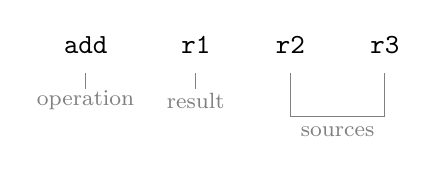
\begin{tikzpicture}[>=stealth]
      \node (op)  at (0,0)   {\ttab{add}};
      \node (rd)  at (1.4,0) {\ttab{r1}};
      \node (rs1) at (2.6,0) {\ttab{r2}};
      \node (rs2) at (3.8,0) {\ttab{r3}};
      \node[smallgraytext] at (0,-0.7) {operation};
      \node[smallgraytext] at (1.4,-0.7) {result};
      \node[smallgraytext] at (3.2,-1.1) {sources};
      \draw[gray] (2.6,-0.35) -- (2.6,-0.9) -- (3.8,-0.9) -- (3.8,-0.35);
      \draw[gray] (1.4,-0.35) -- (1.4,-0.55);
      \draw[gray] (0,-0.35) -- (0,-0.55);
    \end{tikzpicture}
  \end{figure}
  \begin{center}
    \graytext{add the values in \ttab{r2} and \ttab{r3}, and place the result in \ttab{r1}}
  \end{center}
\end{frame}

\begin{frame}
  In this course we use the \highlight{\textbf{MIPS}} instruction set. Each instruction is exactly \highlight{32} bits, split into fields.\\[4mm]
  \begin{figure}
    \centering
    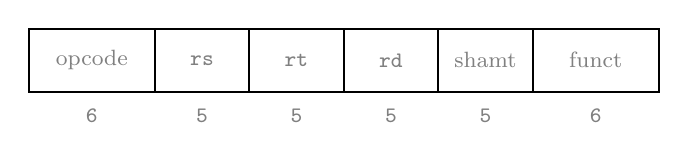
\begin{tikzpicture}[>=stealth]
      \def\w{1.4}
      \foreach \i/\lab/\wid in {0/opcode/1.6, 1/rs/1.2, 2/rt/1.2, 3/rd/1.2, 4/shamt/1.2, 5/funct/1.6} {}
      % draw six fields with their bit widths
      \draw[thick] (0,0) rectangle (1.6,0.8); \node[smallgraytext] at (0.8,0.4) {opcode};
      \node[smallgraytext] at (0.8,-0.3) {\ttab{6}};
      \draw[thick] (1.6,0) rectangle (2.8,0.8); \node[smallgraytext] at (2.2,0.4) {\ttab{rs}};
      \node[smallgraytext] at (2.2,-0.3) {\ttab{5}};
      \draw[thick] (2.8,0) rectangle (4.0,0.8); \node[smallgraytext] at (3.4,0.4) {\ttab{rt}};
      \node[smallgraytext] at (3.4,-0.3) {\ttab{5}};
      \draw[thick] (4.0,0) rectangle (5.2,0.8); \node[smallgraytext] at (4.6,0.4) {\ttab{rd}};
      \node[smallgraytext] at (4.6,-0.3) {\ttab{5}};
      \draw[thick] (5.2,0) rectangle (6.4,0.8); \node[smallgraytext] at (5.8,0.4) {shamt};
      \node[smallgraytext] at (5.8,-0.3) {\ttab{5}};
      \draw[thick] (6.4,0) rectangle (8.0,0.8); \node[smallgraytext] at (7.2,0.4) {funct};
      \node[smallgraytext] at (7.2,-0.3) {\ttab{6}};
    \end{tikzpicture}
  \end{figure}
  \begin{center}
    \graytext{the opcode says what to do, the other fields say which registers to use}
  \end{center}
\end{frame}

\begin{frame}
  There are three formats. They share the opcode but differ in what follows.\\[3mm]
  \begin{figure}
    \centering
    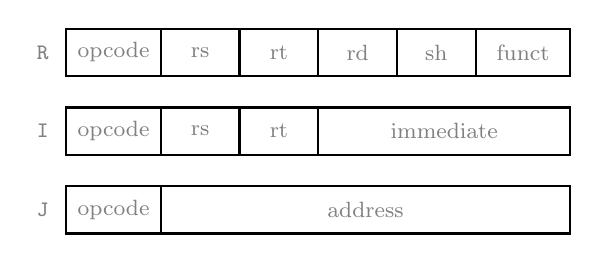
\begin{tikzpicture}[>=stealth, yscale=1]
      % R-type
      \node[left, smallgraytext] at (-0.1,2.4) {\ttab{R}};
      \foreach \x/\ww/\l in {0/1.2/opcode, 1.2/1.0/rs, 2.2/1.0/rt, 3.2/1.0/rd, 4.2/1.0/sh, 5.2/1.2/funct}
        {\draw[thick] (\x,2.1) rectangle ++(\ww,0.6); \node[smallgraytext] at (\x+\ww/2,2.4) {\l};}
      % I-type
      \node[left, smallgraytext] at (-0.1,1.4) {\ttab{I}};
      \draw[thick] (0,1.1) rectangle ++(1.2,0.6); \node[smallgraytext] at (0.6,1.4) {opcode};
      \draw[thick] (1.2,1.1) rectangle ++(1.0,0.6); \node[smallgraytext] at (1.7,1.4) {rs};
      \draw[thick] (2.2,1.1) rectangle ++(1.0,0.6); \node[smallgraytext] at (2.7,1.4) {rt};
      \draw[thick] (3.2,1.1) rectangle ++(3.2,0.6); \node[smallgraytext] at (4.8,1.4) {immediate};
      % J-type
      \node[left, smallgraytext] at (-0.1,0.4) {\ttab{J}};
      \draw[thick] (0,0.1) rectangle ++(1.2,0.6); \node[smallgraytext] at (0.6,0.4) {opcode};
      \draw[thick] (1.2,0.1) rectangle ++(5.2,0.6); \node[smallgraytext] at (3.8,0.4) {address};
    \end{tikzpicture}
  \end{figure}
  \begin{center}
    \graytext{register operations, operations with a constant, and jumps}
  \end{center}
\end{frame}

\begin{frame}
  Registers have names like \ttab{\$t0} and \ttab{\$t1}. A real MIPS add reads two and writes a third.\\[5mm]
  \begin{center}
    \highlight{\ttab{add \$t0, \$t1, \$t2}} \\[3mm]
    \graytext{\ttab{\$t0} $=$ \ttab{\$t1} $+$ \ttab{\$t2}}
  \end{center}
\end{frame}

% ------------------------------------------------------------
% kinds of instructions
% ------------------------------------------------------------
\begin{frame}{Kinds of Instructions}
  \begin{center}
    \Large \highlight{\textbf{kinds of instructions}}
  \end{center}
\end{frame}

\begin{frame}
  Most instructions fall into three groups.\\[3mm]
  \begin{itemize}
    \item \highlight{\textbf{arithmetic and logic}} \\
          \graytext{compute on registers, such as \ttab{add} and \ttab{sub}} \\[2mm]
    \item \highlight{\textbf{data movement}} \\
          \graytext{copy between registers and memory, such as \ttab{load} and \ttab{store}} \\[2mm]
    \item \highlight{\textbf{control flow}} \\
          \graytext{change which instruction runs next, such as \ttab{jump} and \ttab{beq}}
  \end{itemize}
\end{frame}

% ------------------------------------------------------------
% a program
% ------------------------------------------------------------
\begin{frame}{A Program}
  \begin{center}
    \Large \highlight{\textbf{a program}}
  \end{center}
\end{frame}

\begin{frame}[fragile]
  A \highlight{\textbf{label}} marks a position in the program. A control-flow instruction can jump to it, which is how we build loops.\\[3mm]
  \begin{center}
    \begin{lstlisting}[style=myasm]
        li    r1, 0        ; sum = 0
        li    r2, 10       ; i = 10
loop:   beq   r2, r0, done ; if i == 0, leave the loop
        add   r1, r1, r2   ; sum = sum + i
        sub   r2, r2, 1    ; i = i - 1
        jump  loop         ; repeat
done:   store r1, total    ; save the result
    \end{lstlisting}
  \end{center}
\end{frame}

\begin{frame}
  This short program adds the numbers from \ttab{10} down to \ttab{1}. It shows the whole idea of a program:\\[3mm]
  \begin{itemize}
    \item \highlight{\textbf{registers}} \graytext{hold the values being worked on} \\[2mm]
    \item \highlight{\textbf{labels and branches}} \graytext{decide what runs next} \\[2mm]
    \item \highlight{\textbf{memory}} \graytext{keeps the final result}
  \end{itemize}
\end{frame}

% ------------------------------------------------------------
% closing
% ------------------------------------------------------------
\begin{frame}
  \begin{center}
    \Large \highlight{\textbf{the whole stack}}
  \end{center}
\end{frame}

\begin{frame}
  We have built every layer, from the bottom to the top.\\[3mm]
  \begin{figure}
    \centering
    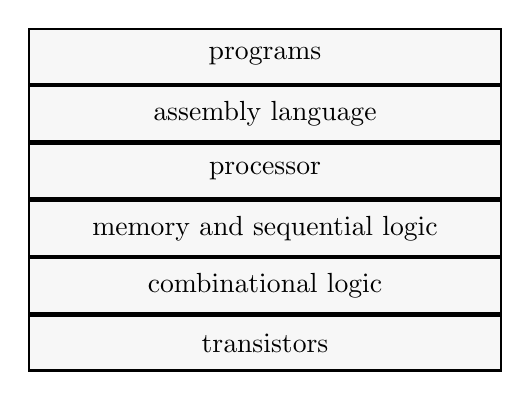
\begin{tikzpicture}[node distance=0mm]
      \tikzset{
        layer/.style={
          draw=black, thick, minimum width=6cm, minimum height=7mm,
          fill=gray!30!white!20, inner sep=0pt
        }
      }
      \node[layer] (l6) at (0,0) {programs};
      \node[layer, below=of l6] (l5) {assembly language};
      \node[layer, below=of l5] (l4) {processor};
      \node[layer, below=of l4] (l3) {memory and sequential logic};
      \node[layer, below=of l3] (l2) {combinational logic};
      \node[layer, below=of l2] (l1) {transistors};
    \end{tikzpicture}
  \end{figure}
\end{frame}

\begin{frame}
  \begin{center}
    A program is just a great many transistors switching in step. That is the whole idea of computer organization.
  \end{center}
\end{frame}

\end{document}
